\documentclass[a4paper,10pt]{report}
\usepackage{fullpage}
\usepackage{setspace}
\usepackage[margin=1.0in]{geometry}
\usepackage[T1]{fontenc}
\usepackage{mathtools}
\usepackage{url}
\usepackage{booktabs}
\usepackage{graphicx}
\usepackage{fancyhdr}
\usepackage{wrapfig}




\begin{document}
\title{3D Procedurally Generated Nature Scene}
\author{Pip Turner - pit@aber.ac.uk \\
Supervisor: Reyer Zwiggelaar\\
G400 Computer Science \\
CS39440}
\date{\parbox{\linewidth}{\centering%
  \today\endgraf\bigskip
  \textit{Version 1.0}
  }}
\maketitle

\setlength{\headheight}{20.2pt}
\pagestyle{fancy}
\setlength{\headsep}{0.2in}
\fancyhf{}

\fancyhead[L]{\leftmark}
\fancyhead[R]{\rightmark}

\fancyfoot[CE,CO]{\leftmark}
\fancyfoot[LE,RO]{\thepage}

\listoffigures
\listoftables

\tableofcontents
\clearpage



\section{Abstract}
3D Procedural Generation is a way to produce high variety 3D models quickly without manually creating the content. This Project is going to focus on the implementation and subsequent levels of variation of Procedural Generation Algorithms in order to create a cohesive scene. I will be focusing on creating nature based content, e.g. Terrain, Trees and Foliage in order to combine them together and create a dense scene which also renders smoothly. 
\clearpage
\chapter{Introduction}
\section{Project Description}

Procedural Content Generation is a broad term referring to the creation of content automatically through algorithmic means~\cite{yannakakis2011experience}. The most popular examples of Procedural Generation are usually the use of it in creating Procedurally Generated Worlds, such as No Man's Sky~\cite{nomanssky} - a game which provides the player with a procedurally generated universe to explore. Projects which aim to generate entire planets, or even universes are what initially made me interested in procedural generation - the vast scope, potential and variety of  scenes excited me the most. \\


\begin{figure}[h!]
    \centering
  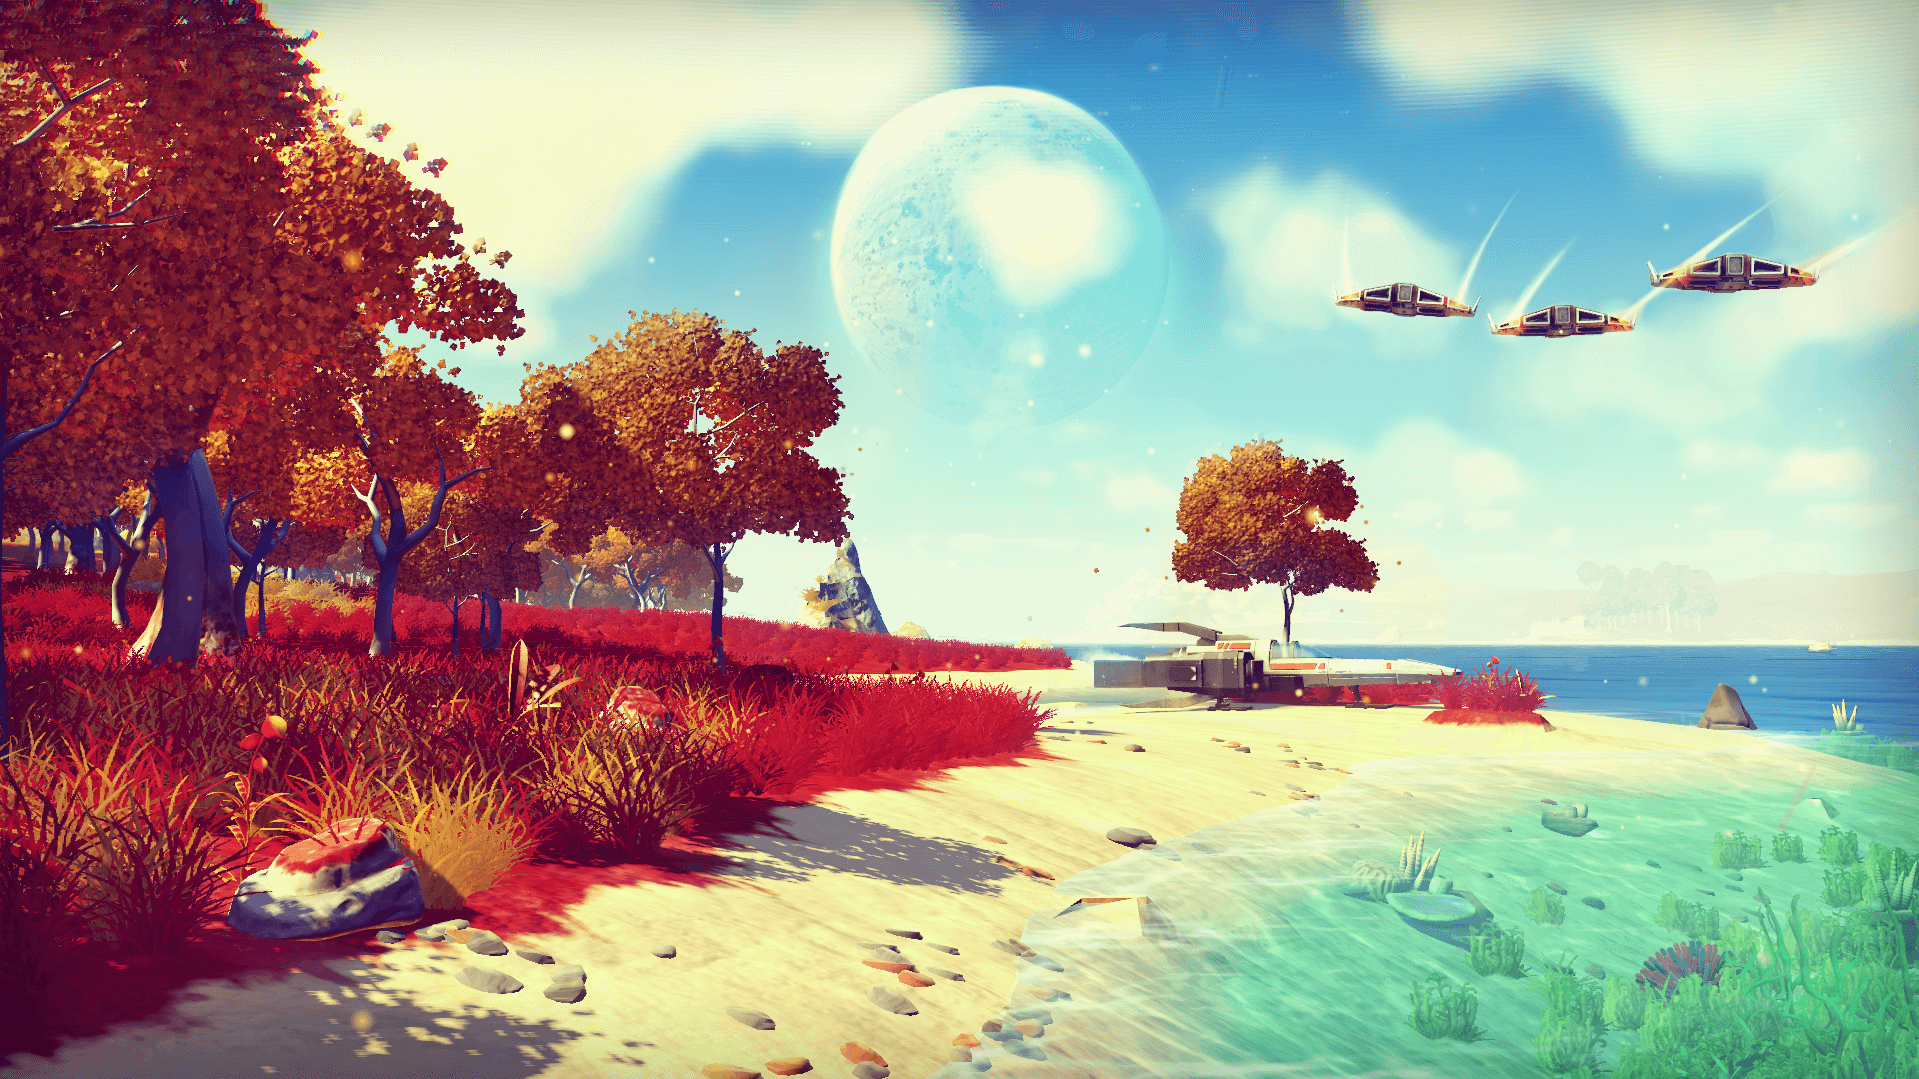
\includegraphics[width=0.9\textwidth]{NoMansSky}
 \caption{No Man's Sky. Source: https://www.nomanssky.com/press/}
 \label{fig:no_mans_sky}
\end{figure}


This project, therefore is a 3D Procedurally Generated Nature Scene - a small, dense scene utilising procedural content generation techniques to create a  scene which is visibly different each time it is generated. \\

However, my knowledge of all areas of this project was limited when beginning - this project is as much a personal opportunity to learn low level 3D Graphics and Procedural Generation techniques as it is simply an exercise in implementing them. 

\section{Project Aims}
The aims of the project are as follows:\\

\textbf{\textit{Create a 3D Procedurally Generated Nature Scene}} \\

The heart of this project is creating a 3D nature scene which is different each time it is generated, using 3D Procedural Content Generation. Rather than creating large, vast swathes of land, I am instead aiming for a smaller, dense scene in order to generate more interesting landscapes. The smaller the scene, the less content is needed to be generated in order to ensure high levels of variation.\\

The main work involved in this aim will be the implementation and subsequent optimisation and use of procedural algorithms. The basic two ingredients needed are Terrain and Trees - this would at the very least show a good understanding and implementation of two to three procedural algorithms. Once these are well implemented, I can add foliage and other details in order to increase the variety of the scene, further progressing the detail and complexity of the scene.  \\


\textbf{\textit{Become competent with C++, OpenGL and the core fundamentals of low level graphics}} \\

The other main aim of this project is in regards to the skills and technologies learnt whilst working on it. I have begun this project with a basic understanding of C++, basic ideas about procedural generation algorithms and no understanding of OpenGL (albeit some basic knowledge of graphics and graphics libraries). In aiming to achieve this project, I hope to come out of it with a greater appreciation and understanding of C++, procedural generation algorithms and OpenGL.\\

\chapter{Research}

In researching into this project, I needed to clearly find and choose suitable algorithms. In selecting them, I narrowed them down into two categories - Terrain and Objects on the Terrain. \\

\section{Existing Solutions}

\subsection{Terrain}

A major part of this project was selecting and subsequently implementing a terrain algorithm which produced suitably varied and realistic looking terrain. One of the most popular noise generation techniques for Procedural terrain is Perlin Noise~\cite{perlin2002improving} - an algorithm which has been widely used for 3D Graphics, and something which has been instrumental in improving 3D graphics. Whilst it is a popular algorithm, it can be quite computationally expensive and difficult to implement in comparison to other algorithms.\\

My supervisor, Reyer Zwiggelaar, suggested looking into Fractal Images, initially suggesting some realistic natural growth based algorithms~\cite{Bilsborough3424}. One of the most widely used Fractal Terrain algorithms is Diamond Square~\cite{olsen2004realtime} - a variation on midpoint displacement. Midpoint Displacement's main issue was that when generating a heightmap it often left "creases" in its landscape, an issue Diamond Square aims to fix by using two stages of midpoint displacement - named Square and Diamond.  \\

\begin{figure}[h!]
    \centering
  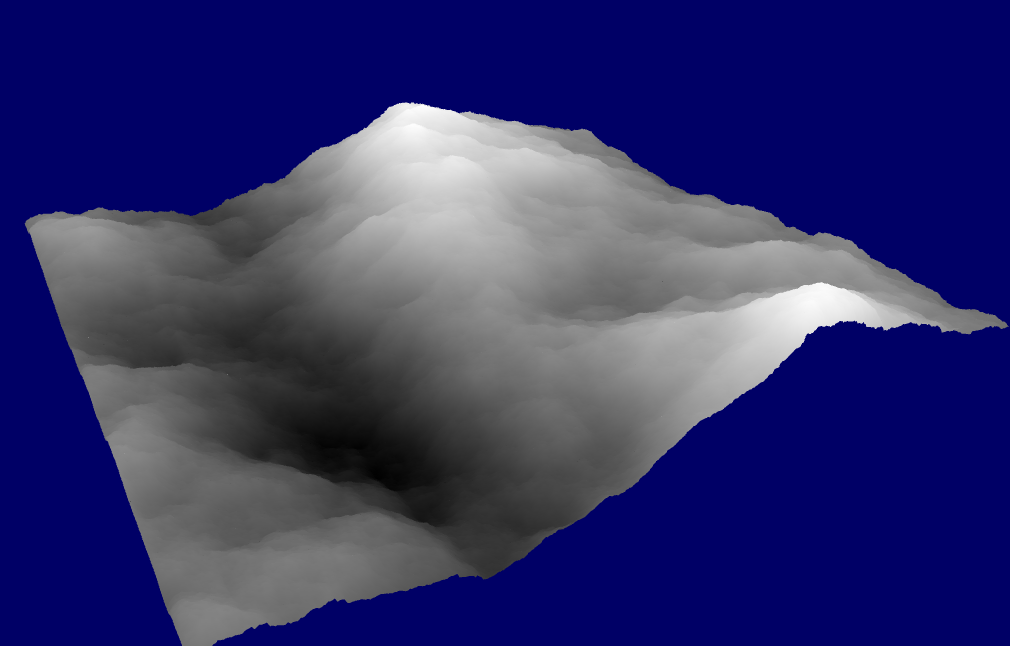
\includegraphics[width=0.5\textwidth]{DiamondSquareGreyScale}
 \caption{Diamond Square Terrain with a Greyscale colour applied to it}
 \label{fig:DiamondSquareGrey}
\end{figure}

\subsection{Objects on Terrain}

As well as procedural terrain, in order to ensure a high level of variety objects upon the terrain are going to also need to be generated. This project will focus mainly on foliage, i.e. Trees, plants and grass. In researching procedurally generated trees I identified two methods which I could implement - Lindenmayer Systems~\cite{lindenmayer2017} or a Space Colonisation Algorithm~\cite{runions2007modeling}. 

\textbf{\textit{CITE Fractals and Chaos}}\\
Lindenmayer System is a fractal generation algorithm which builds a fractal by iterating over a string, following a ruleset~\cite{prusinkiewicz2012algorithmic}. The string can then be interpreted into something drawable. This allows for infinite number of unique fractal patterns to be generated, but most importantly, it can be used to generate trees, bushes and grass like fractals.  

Space Colonisation~\cite{runions2007modeling} works by defining an area in space, filling it with "seeds" (points in space) and "growing" branches towards those points. By doing this, it becomes an incredibly powerful tree generator - generating a huge variety of trees depending on the defined area and the amount of seeds.

\subsection{Optimisation}
This project will require displaying a lot of objects and vertices at once, meaning that optimisation techniques will need to be implemented, as the more vertices on the screen, the lower the framerate. In order to display the scene professionally, we need to aim for a high framerate (between 30 and 60).  \\

There are a number of big optimisations associated with 3D Graphics. The most applicable optimisation to both Terrain and Trees is Level Of Detail. The further the way an object is from the user, the less detailed the object needs to be. For example, if the player is looking at a far off Mountain, they won't be able to see all of the nooks and crannies on it, only the general shape. This means that we can severely decrease the number of vertices on objects which are far away, whilst keeping high detail on objects which are closer. \\

Level of Detail is even more relevant when displaying objects like trees, bushes and grass. We can go even further with these using Billboards and Impostors~\cite{jia2013fast}. The basic premise of them is if the tree is far enough from the player for the player to not realise, we can generate an image of the tree and display the image instead. For Example, if we have a tree with five hundred vertices, we can simply display it using six, by mapping the image of the tree onto a quadrilateral polygon made up of two triangles. These images can differ depending on how far away the object is from the player. If the object is very far, we can simply display one image of it, oriented towards the player - this is known as Billboarding. However, if the object is a bit closer to the player, we can display an image of the tree at a certain rotation, giving the illusion of perspective to the player. The implementation of Billboards and Impostors can also vary from object to object. Grass, as it is so small can potentially simply be displayed as a Billboard for all of its lifetime. Billboards and impostors can provide huge optimisations, drastically cutting down the number of polygons in the scene whilst maintaining the illusion of density. \\

Objects on the Terrain can also be optimised using instancing and by implementing the Flyweight Design Pattern (\emph{see section 1.5.4}). Instance Rendering allows us to draw the same tree multiple times in different places, whilst only ever storing the data of it once. This saves hugely on memory space.  


\subsection{Design Patterns}

There were no Architectural Design Patterns which seemed relevant for this project. Model View Controller~\cite{vlissides1995design} was considered, but when implementation was theorised, it was found that the pattern simply didn't fit this project - it would be overkill to implement a pattern which lent so heavily on a database on a project which doesn't require any database functionality. \\

However, I have identified two programming patterns which are relevant to my project: Flyweight and Command~\cite{nystrom2014game}.\\

\emph{\textbf{Flyweight}}\\

Flyweight allows you to share common information between objects. This is hugely useful for Trees - they may have the same mesh, colour details or texture. Separating out this data, and then having the instances of the trees carry a pointer to the data can allow for optimised data sharing. \\

\emph{\textbf{Command}}\\

Command can be used for different inputs the player makes. Instead of hardcoding each keypress, we can implement command, which abstracts the keypress from the command, allowing for easy remapping of keys. This can come in useful for handling movement within the program. 

\section{Suitability of Algorithms}

\subsection{Terrain}

For Terrain, I am going to use the Diamond Square algorithm. As I am coming to this project with limited initial knowledge, choosing an algorithm which is relatively simple to implement, and which produces similar results to Perlin noise is preferable. As Diamond Square is less complex, it also takes less time to generate its height map. However, in comparison to Perlin Noise, it is less flexible - Perlin Noise can be used to generate infinite surroundings on the fly, needing no knowledge of points next to it, whereas Diamond Square Terrain needs to be generated as a whole before it is rendered, meaning that chunks would have to be stitched together to create infinite terrain. However, as the aim of this project is not to provide infinite terrain, but rather a variation on a small part of Terrain, this is not too much of an issue for me. 

\subsubsection{Objects}

When adding objects to my terrain, I hope to have a high level of variety. As the time on this project is limited, I have decided to use Lindenmayer Systems over Space Colonisation. In using L-Systems, I can have a high range of different fractals, providing an interesting scene to look at. Lindenmayer Systems are not only fast and have a low memory footprint, they allow for huge variation in not just trees but in creating other objects such as plants, grass and bushes. 

\section{Proposed Implementation}
\subsection{Overview}

In creating this project, it is not only the software implementation which is important to consider, but also the development life-cycle as a whole. A well planned life-cycle can make or break a project. 

\subsection{Software Development}
\subsubsection{Life-cycle}

An Agile Methodology seemed well suited to the project, as the technologies were so new to me, and the project so dynamic in scope. Following a Waterfall style system wouldn't have worked as well, as I wouldn't have been able to plan effectively, due to lesser knowledge of the subject. Agile Methodologies tend to be less rigidly structured, allowing me more flexibility to learn and experiment within the project. \\

With this in mind, I chose to use a One Man Scrum Methodology. In a One Man Scrum tutorial, written by Alex Andrews,~\cite{andrews_2017} Andrews discusses the core principles of Scrum - Shipping features regularly, productivity and self reflection \& meaningful iteration. Scrum works by splitting development up into short sections known as "Sprints". Features of a program which need implementing are known as Stories, and each Sprint is focused around completing a specific set of stories, decided upon before the sprint began. \\

\begin{figure}[h!]
    \centering
  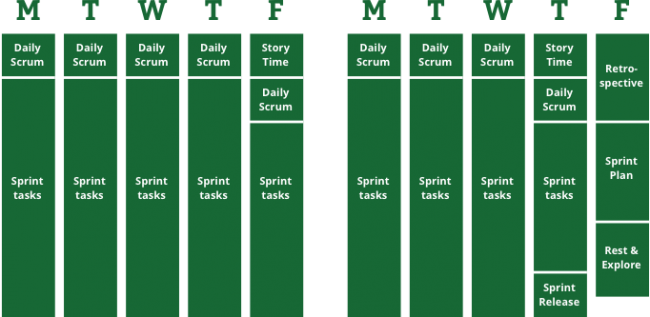
\includegraphics[width=0.9\textwidth]{RayWenderlich}
 \caption{A proposed two week Sprint plan by Alex Andrews, sourced from https://www.raywenderlich.com/162654/scrum-one-bring-scrum-one-person-operation . Used with permission.}
 \label{fig:two_week_sprint_plan}
\end{figure}

As seen in Figure~\ref{fig:two_week_sprint_plan}, Andrews proposes a two week Sprint, each day featuring a Daily Scrum, followed by completion of sprint tasks. Each week ends with Story Time, with the final week ending with a Retrospective, Sprint Plan and a time for exploration. Whilst I liked the general layout of the two weeks, I had to adapt it to my own project, as I had less time compared to Andrews. \\

\begin{figure}[h!]
    \centering
  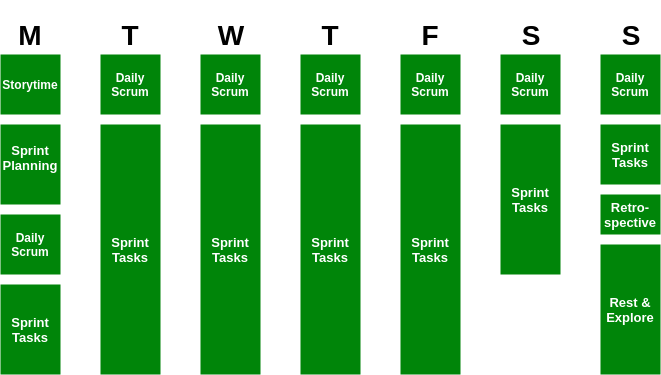
\includegraphics[width=0.9\textwidth]{Sprint_Plan}
 \caption{An adapted version of Alex Andrew's One Man Two-Week Sprint}
 \label{fig:one_week_sprint_plan}
\end{figure}

In Figure~\ref{fig:one_week_sprint_plan}, Andrew's Sprint was adapted into a one week solution, which spanned the entire week rather than five days. \textit{Sprint Release} was removed as the project wouldn't be releasing  releasing to would be myself, so I could build up commits and features throughout the week. I moved Story planning and Sprint planning to the beginning of the week, to ensure a more focused week throughout. On top of this, my retrospective and exploration were moved to Sunday. \\

To support this, I kept a Sprint Log alongside my projects development, which was essentially a record of my daily scrum. Each day I kept a record of my intentions for the day, making sure to relate them to the stories planned and recorded on the Monday. This worked well, as Mondays also tended to be the day I met with my project's supervisor \& the day I assigned for Write-Up. Having Monday as a planning and Write Up day gave me a good sense of motivation and a good chance to rest from programming. \\

Whilst I am doing an Agile Methodology, it does not mean that  project planning as a whole can be dismissed. On top of planning at the start of my Sprints, I also used a Gantt Chart to make sure I was on track with both Write Up, Sprints and Project deadlines. This, coupled with the Project Outline Spec, gave me a lot of insight into how I was going to shape the project, and ensure that it would be finished on time. \\

\section{Relevant Technology}

\subsection{C++}

This project will be coded primarily in C++, as an aim of the project is to become more familiar and more comfortable with C++. As well as this, C++ has its own benefits - it tends to be very fast, is very often used for graphics coding due to the powerful libraries available, such as DirectX~\cite{directx_website}, OpenGL~\cite{opengl_website} and Vulkan. When writing in C++, I aimed to follow Google's Style Guide's~\cite{google_c_style_guide} naming conventions, in order to ensure a coherent and consistent code base.

\subsection{OpenGL}
In choosing C++, I had a lot of Graphics APIs to choose from. I disregarded DirectX's Direct3D due to its limited application in terms of cross platform - it only being compatible with Windows based hardware. Vulkan, intended to be a "Next Generation OpenGL" was also eventually disregarded as an option. Despite being newer, and potentially more powerful than OpenGL, it is also more verbose and therefore harder to pick up. As I am relatively new to 3D Graphics APIs, having only used high level JavaScript libraries beforehand, it was more advisable for me to use OpenGL - a cross platform graphics API. Using OpenGL gives me a better way to learn the fundamentals of low level graphics, as well as the option to move onto Vulkan in the future.

\subsection{GLSL}

GLSL, or \textit{OpenGL Shading Language} is the language used by OpenGL for its shaders. Whilst I won't be focusing too much on shaders for this project, they are still needed by necessity, and so some GLSL will be used.

\subsection{CLion}
I chose to use CLion~\cite{clion_jetbrains} as my IDE of choice, it offers powerful tools for a programmer, as well as a very slick user interface. Having used and enjoyed Jetbrains products previously, using CLion for this project seemed like an obvious choice.

\subsection{LaTeX}
In order to write this report, I chose to use LaTeX~\cite{latex_website}, due to its professional rendering of documents. I used overleaf.com~\cite{overleaf_website}, a cloud based LaTeX editor to edit my report in, which ensured that my data couldn't get lost.

\subsection{Draw.io}
Any chart used in this document were generated using draw.io~\cite{draw_io}, an easy to use chart maker, which gave me the option to save to cloud based providers, again allowing me to easily keep my data safe. 

\subsection{Version Control - Git \& Github}
This project was made using Git as version control, being saved to a private repository on Github~\cite{github}. This allowed easy rollbacks where needed, as well as ensuring that my data would not be lost, as it is saved on the cloud. In addition to this, Overleaf was used for version control and cloud saving for the report - it also uses a Git backend for this.


\chapter{Design and Implementation}

\section{Software Structure}
As my project is so reliant on C++ and OpenGL, these two technologies dictate my Software's structure. C++ is primarily an Object Oriented Language, with OpenGL being a state machine and Graphics API, a structure already built into it. 
\section{Algorithms}
\subsection{Diamond Square}
The Diamond Square algorithm~\cite{miller1986definition}, is an algorithm which randomly generates fractal based terrain, iterating over terrain using two steps - Diamond and Square. \\ 

\begin{figure}[h!]
    \centering
  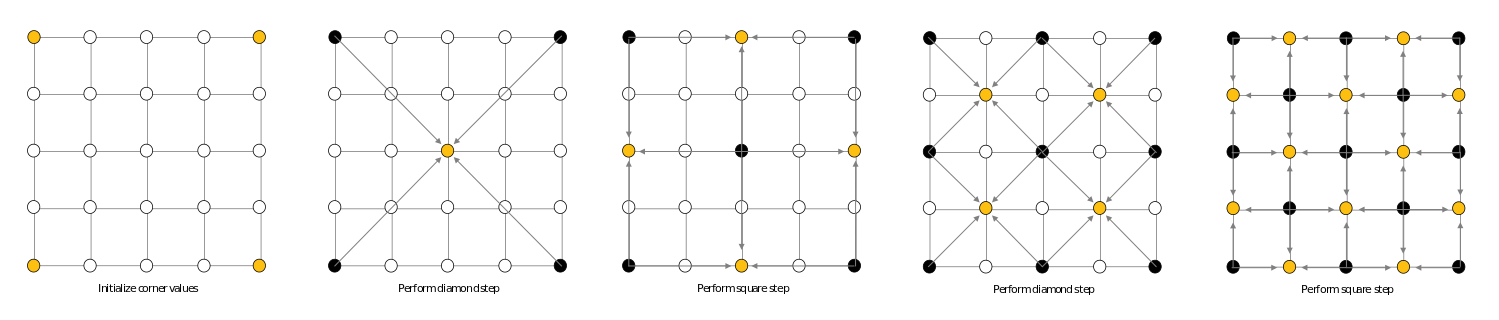
\includegraphics[width=0.9\textwidth]{Diamond_Square}
 \caption{Diamond Square steps, by Christopher Ewin CC BY-SA 4.0, https://commons.wikimedia.org/w/index.php?curid=42510593}
 \label{fig:diamond_square_steps}
\end{figure} 

Diamond Square is performed on an initially flat grid. The steps (as pictured in fig~\ref{fig:diamond_square_steps}) are as follows:

\begin{enumerate}
\item \textit{Initialise corner values}
\item \textit{Diamond Step}
\item \textit{Square Step}
\item \textit{Reduce step size} 
\item \textit{Repeat Steps 2-4 while step size is greater than 1}
\end{enumerate} 

The Step Size (used in both the Square Step and the Diamond Step) is initialised to the grid's width -1. The Diamond step takes each square in the grid, of width Step Size, and sets the midpoint of the square to the average of its corner values, in addition to a random value (which decreases alongside Step Size). The Square step takes each diamond in the gird of width Step Size and sets the midpoint of the diamond to the average of its corner values, in addition to a random value (which decreases alongside Step Size). \\

One of the main issues with Diamond Square are edge values - whilst all other values gain their height from the average of 4 other values, edge cases don't have enough data around them for this. There are two solutions to this - use the 3 available values, or wrap round the values to the other side of the grid. 

\subsection{Lindenmayer Systems}

Lindenmayer System is a String manipulation algorithm, which recursively iterates over a String according to a set of rules in order to generate a String representation of a fractal pattern. It's steps are as follows:

\begin{wrapfigure}{r}{4cm}
\centering
  \fbox{
\includegraphics[width=0.11\textwidth]{AB_Example.png}}
 \caption{Diagram illustrating an L-System's iterative process}
 \label{fig:l_system_AB}
\end{wrapfigure}

1. Define initial String seed
2. Define the L-System's rules
3. Iterate over the string \textit{n} times, following the defined rules


A simple example:\\

\textbf{Seed:} \textit{"A"}

\textbf{Rule 1:} \textit{A $\rightarrow$ AB}

\textbf{Rule 2:} \textit{B $\rightarrow$ A}


Iteration 0: A

Iteration 1: AB

Iteration 2: ABA

Iteration 3: ABAAB

Iteration 4: ABAABABA

Iteration 5: ABAABABAABAAB\\



In Figure \ref{fig:l_system_AB}, Patterns can be generated easily and quickly. The next stage of Lindenmayer Systems is interpreting these patterns into something we can draw - this is achieved using "Turtle Graphics". The book, The Algorithmic Beauty of Plants~\cite{prusinkiewicz2012algorithmic} contains a comprehensive explanation of Lindenmayer Systems including these rules for 3D Lindenmayer Patterns:\\

F: Move forward, by step \textit{d} and orientation \textit{n}. A line between {x, y, z} and {x', y', z'} is drawn.

f: Move forward, by step \textit{d} and orientation \textit{n}. 

+: Turn left by angle $\sigma$ along the xy axis (using the z rotation matrix)

-: Turn right by angle $\sigma$ along the xy axis (using the z rotation matrix)

\&: Pitch down by angle $\sigma$ along the xz axis (using the y rotation matrix)

$\wedge$: Pitch up by angle $\sigma$ along the xz axis (using the y rotation matrix)

\textbackslash: Roll left by angle $\sigma$ along the yz axis (using the x rotation matrix)

/: Roll right by angle $\sigma$ along the yz axis (using the x rotation matrix)

|: Turn around along the xy axis (180 degrees using the z rotation matrix)

[: Push the current state of the turtle onto a stack

]: Pop a state from the stack and apply it to the turtle\\

These rules expand the usefulness of Lindenmayer Systems. [ and ] especially are useful for this project, as they allow for branching structures, allowing us to create trees.

\clearpage
\subsection{Terrain LOD}

\begin{figure}[h!]
    \centering
  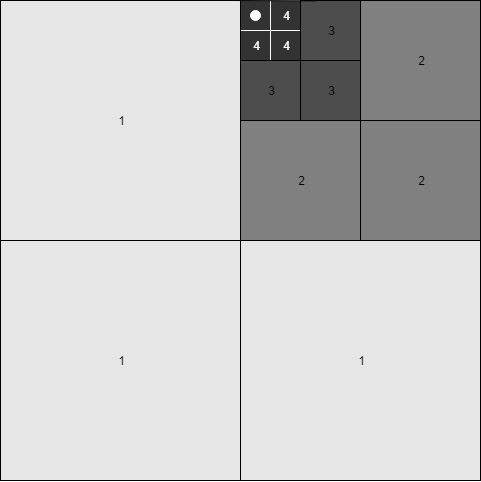
\includegraphics[width=0.3\textwidth]{QuadTree.png}
 \caption{Quadtree example. The darker the shade, the higher detailed the terrain in that area. White circle denotes where the camera is.}
 \label{fig:quad_tree}
\end{figure}

One of the biggest optimisations to be made for this project will be Terrain Level Of Detail (LOD). This optimisation is split into two parts - the generation of the different levels of detail, alongside the combining of them, and deciding the amount of vertices to display. This could be done dynamically, but lacking the time and definition  to implement the complexity of a dynamic terrain renderer, instead we have something easier to use. Diamond Square, upon generating its terrain automatically generates different levels of detail which can easily used for this algorithm. These levels of detail can then be stitched together, depending on the technique used for LOD display. \\

An often used technique for deciding what LOD each chunk of terrain will be is using a Quad Tree system to split up terrain~\cite{pajarola1998large}. A Quad Tree is a tree structure where each node has exactly four children. As seen in Figure~\ref{fig:quad_tree}, this tree structure can easily be applied to splitting up terrain. In Figure~\ref{fig:quad_tree}, each shade (as denoted by the numbers) represents a different Level Of Detail - the darker the shade, the higher the detail. whilst this can easily work, the main problem are cracks between each chunk of terrain. This can potentially be solved by working averaging the edges to the midpoint of each other, but this could potentially prove problematic as each edge has different numbers of triangles. A crude solution would involve moving the edge vertices of the edge triangles up to the same elevation as the edge of their neighbouring chunk. \\

A solution to this problem is known as Restricted Quadtree Triangulation~\cite{pajarola1998large}. This works by restricting triangulation to points that match. Whilst this is definitely a more elegant method, I am unsure if I will have the time to implement it. 

\subsection{L-System Rendering Optimisation Techniques}
L-Systems when displayed on screen may use a lot of vertices, especially if displayed using 3D Primitives such as cylinders. In order to reduce the amount of vertices displayed we can use a similar technique to Terrain LOD. 


\chapter{Sprints}
\section{Sprint 1 (12/02/18 - 18/02/18)}
\section{Sprint 2 (19/02/18 - 25/02/18}
\section{Sprint 3 (26/02/18 - 04/03/18)}
\section{Sprint 4 (05/03/18 - 11/03/18)}
\section{Sprint 5 (12/03/18 - 18/03/18)}
\section{Sprint 6 (19/03/18 - 26/03/18)}
\section{Sprint 7 (26/03/18 -  01/04/18)}
\section{Sprint 8 (02/04/18 -  09/04/18)}
\section{Sprint 9 (10/04/18 -  17/04/18)}

\chapter{Tests}

\chapter{Results}
\section{Analysis}
\subsection{Implementation Challenges}
\subsection{Overall Problems and Issues}
\section{Future Additions}

\chapter{Conclusion and Evaluation}
\section{Evaluation}
\subsection{Project Aims}


\clearpage
\bibliographystyle{IEEEannot}
\bibliography{bibliography.bib}
\end{document}